\chapter{Desenvolvimento do DiaVision}
\label{ch:development}

Neste capítulo são apresentadas as tecnologias utilizadas, as soluções adotadas para os problemas
de acessibilidade identificados no MSL e os resultados alcançados ao final do processo desenvolvimento.

\section{Tecnologias Utilizadas}

Esta seção lista as principais tecnologias e recursos utilizados no desenvolvimento do sistema DiaVision.

\subsection{Visual Studio Code}

O Visual Studio Code (VSCode) é um editor de código \emph{open source} desenvolvido pela Microsoft para Windows, Linux e MacOS.
Ele inclui suporte para depuração, controle de versionamento Git incorporado, realce de sintaxe, IntelliSense
- termo para um conjunto de funcionalidades de edição de código, tais como completar código e informações de parâmetros -
e refatoração de código.

O VSCode também possibilita a instalação de extensões que adicionam funcionalidades ao editor, assim, aumentando a produtividade do desenvolvedor.
Por conta dessas características, esse foi o editor utilizado neste projeto tanto para desenvolver o sistema DiaVision quanto para a parte escrita deste trabalho.

As extensões utilizadas para desenvolvimento da aplicação foram: Flutter e Dart, que dão suporte à criação de aplicações com o SDK do Flutter
e fluttermobx, que oferece atalhos para adicionar componentes de gerenciamento do estado da aplicação. Já Para a parte escrita,
foi utilizado o conjunto de extensões: bibtexLanguage, Code Speell Checker, LaTeX e LaTeX Workshop.

\newpage

\subsection{Github}

O Github é uma plataforma de desenvolvimento e gestão de código-fonte, baseada no Git, que permite aos usuários compartilhar seus projetos e arquivos com controle
de versionamento de código. Com isso é possível realizar \emph{commits}, sendo cada \emph{commit} um ponto de alteração no histórico do
projeto, criar \emph{branches}, ramificações que possibilitam trabalhar em diferentes funcionalidades ao mesmo tempo e realizar \emph{merges},
que é processo de unir ramificações.

O versionamento de código é uma das funcionalidades mais importantes do Git, pois, manter o histórico de alterações
facilita a investigação e resolução de problemas e, em caso de falhas em uma versão do projeto, é possível reverter para uma
versão anterior.

O Github é gratuito e permite a criação de projetos públicos e privados, porém, os repositórios privados possuem limitações
nas funcionalidades da plataforma. Ambos os repositórios, do desenvolvimento do DiaVision\footnote{\url{https://github.com/jnthnklvn/dia_vision}}
e da parte escrita com LaTeX\footnote{\url{https://github.com/jnthnklvn/tcc_dia_vision}} subiram para o GitHub,
inicialmente de forma privada e disponibilizados de forma pública após a finalização deste trabalho.

\subsection{Ambiente de Desenvolvimento}

A máquina principal utilizada para desenvolvimento do sistema DiaVision foi um computador de mesa (do inglês \emph{Desktop}), com o SO Windows 11.
Porém, trata-se do desenvolvimento de uma aplicação multiplataforma e não é possível testar a aplicação para o sistema operacional
iOS, da Apple, em um computador que não seja esteja rodando o macOS. Assim, para validação do aplicativo, também foi
utilizado um MacBook.

O \autoref{qua-esp-maq-gui} mostra as especificações das máquinas utilizadas no desenvolvimento do sistema.

\begin{quadro}[htb!]
    \begin{center}
        \ABNTEXfontereduzida
        \caption{\label{qua-esp-maq-gui}Máquinas de Desenvolvimento.}
        \begin{tabular}{|c|c|c|}
            %\hline
            \hline
                                & \textbf{\emph{Desktop}}  & \textbf{MacBook}        \\
            \hline
            Sistema Operacional & Windows 11 Pro 22H2      & macOS Big Sur 11.3.1    \\
            \hline
            Disco Rígido        & SDD NVMe 512GB e HD 1TB  & 256GB SDD               \\
            \hline
            Memória RAM         & 32GB 3000MHz DDR4        & 8GB 1600MHz DDR3        \\
            \hline
            Processador         & AMD Ryzen 5 5600X 6-Core & Intel Core i5 Dual-Core \\
            \hline
            % \hline
        \end{tabular}
        \legend{Fonte: Autor.}
    \end{center}
\end{quadro}

\subsection{Dispositivos de Teste}

Os testes e validações da aplicação, durante o processo de desenvolvimento, foram realizados em dispositivos físicos
rodando o SO Android, porém, para o iOS os testes foram realizados por meio do iOS Simulator, disponível apenas em
computadores com o SO macOS.

Assim, o \autoref{qua-esp-smart} apresenta as especificações dos \emph{smartphones} utilizados durante o desenvolvimento
do aplicativo.

\begin{quadro}[htb!]
    \begin{center}
        \ABNTEXfontereduzida
        \caption{\label{qua-esp-smart}\emph{Smartphones} utilizados no Desenvolvimento.}
        \begin{tabular}{|c|c|c|}
            %\hline
            \hline
                                  & \textbf{Galaxy S20} & \textbf{Redmi Note 8}   \\
            \hline
            Marca                 & Samsung             & Xiaomi                  \\
            \hline
            Sistema Operacional   & Android 12          & Android 9.0             \\
            \hline
            Armazenamento Interno & 128GB               & 32GB                    \\
            \hline
            Memória RAM           & 8GB                 & 3GB                     \\
            \hline
            \emph{Chipset}        & SAMSUNG Exynos 990  & Snapdragon 665 Qualcomm \\
            \hline
            % \hline
        \end{tabular}
        \legend{Fonte: Autor.}
    \end{center}
\end{quadro}

\subsection{Back4app}

O Back4app é uma plataforma gratuita (no plano básico) que segue o modelo de serviço em nuvem \emph{Backend} como Serviço (BaaS, do inglês \emph{Backend as a Service})
para desenvolvimento de \emph{backend} e gerenciamento de infraestrutura com eficiência e facilidade. Com a plataforma é possível
criar estruturas de dados e serviços de forma simples, sem a necessidade de codificação, possibilitando também a adição de código por meio de \emph{Cloud
    Functions}\footnote{Com Funções em Nuvem é possível escrever funções simples que são disparadas a partir de eventos emitidos
    pela infraestrutura e serviços de nuvem.} para criar validações ou funcionalidades mais complexas.

A plataforma é baseada no ParsePlatform, um \emph{framework} de código aberto que fornece um conjunto de SDKs que visam a criação rápida de \emph{backends}
com armazenamentos de objetos e arquivos, autenticação de usuário, \emph{push notifications}, \emph{dashboard} para gerenciamento e integração com aplicações móveis e \emph{web}.

O Back4app também disponibiliza a criação, customização e hospedagem de uma aplicação \emph{web} para administração do sistema.
Sendo possível definir as classes e operações que estarão disponíveis para gerenciamento pelo administrador do sistema.

Devido a simplicidade que o Back4app oferece para criação, gerenciamento e hospedagem de \emph{backend}, comparado
à aplicações convencionais desenvolvidas por meio da codificação, e ao foco deste trabalho, que é o
desenvolvimento da aplicação móvel com o foco na usabilidade, esse foi o serviço escolhido para o desenvolvimento do sistema.

O plano utilizado para o serviço foi o gratuito, que possui limite de 10 mil requisições por mês, 250MB para armazenamento de dados,
1GB para transferência de dados, 1GB para armazenamento de arquivos e 1 \emph{Cloud Code Job}\footnote{\emph{Cloud Jobs} são utilizados
    para execução de funções de longa duração, das quais não é necessário aguardar a resposta, no servidor. Em outras soluções é possível
    executar essas funções periodicamente, porém, essa funcionalidade ainda não está disponível no Back4app e elas precisam ser disparadas
    por meio da API Rest.}.

\subsection{Flutter}

O \emph{framework} escolhido para desenvolvimento do aplicativo móvel foi o Flutter, apresentado no Capítulo \ref{ch:fundament},
devido a sua facilidade no desenvolvimento móvel multiplataforma, possibilitando a geração de aplicações
para Android e iOS a partir de uma base de código única, mantendo desempenho próximo ao de aplicações nativas.

\section{Implementação}

Esta seção detalha as soluções de implementação adotadas, tais como a arquitetura do sistema e as soluções
para os problemas de acessibilidade.

\subsection{Organização e Estrutura do Projeto}

A estrutura de pastas do projeto está organizada em módulos, os quais não conhecem uns aos outros,
apenas as classes relativas ao próprio módulo estão dentro de cada pasta. A exceção é para os \emph{repositories} (repositórios)
que estão numa camada separada e contém os modelos e as conexões com a fonte de dados.
Essa camada não tem conhecimento a respeito das demais camadas da aplicação.

\newpage

Dentro de cada módulo estão as outras duas camadas, os \emph{controllers} (controladores) e a \emph{view} (interface visual).
Os \emph{controllers} fazem a mediação entre a \emph{view} e os \emph{repositories}, eles controlam o estado da aplicação,
devendo atualizar a \emph{view} quando receber atualização dos \emph{repositories} e chamar os \emph{repositories}
quando algum evento é disparado na \emph{view}.

A \autoref{fig_est_proj} mostra como está organizada essa estrutura de pastas, sendo que a \emph{view}
está divida em \emph{pages}, que são as telas e \emph{widgets}, que são os componentes que fazem parte das telas.

\begin{figure}[htb]
    \caption{\label{fig_est_proj}Estrutura de Pastas do Projeto.}
    \begin{center}
        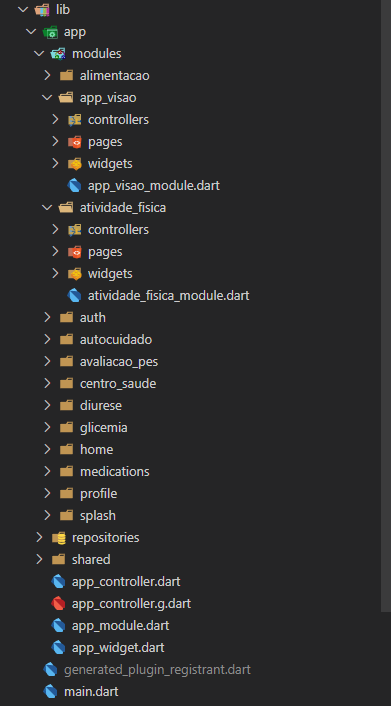
\includegraphics[scale=0.75]{Imagens/desenvolvimento/arquitetura_dia_vision.png}
    \end{center}
    \legend{Fonte: Autor.}
\end{figure}

Ainda na \autoref{fig_est_proj} percebe-se que dentro de cada módulo existe uma classe geral, é nela onde são definidas
as rotas, injeções de dependências e \emph{singletons}\footnote{\emph{Singleton} é um padrão de projeto que garante
a existência de apenas uma instância de uma classe.} de cada módulo, como mostra a \autoref{fig_mod_app_vis}.

\newpage

\begin{figure}[htb]
    \caption{\label{fig_mod_app_vis}Classe Principal do Módulo.}
    \begin{center}
        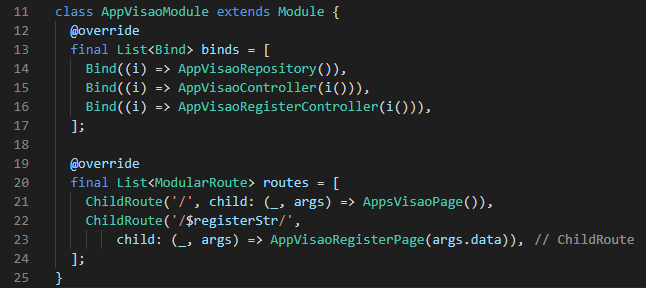
\includegraphics[scale=0.7]{Imagens/desenvolvimento/app_visao_module.png}
    \end{center}
    \legend{Fonte: Autor.}
\end{figure}

Os \emph{singletons} dos repositórios são injetados nos construtores dos controladores como mostrado nas linhas 15
e 16 da \autoref{fig_mod_app_vis} e recuperados pelos controladores conforme mostrado na \autoref{fig_con_app_vis}.

\begin{figure}[htb]
    \caption{\label{fig_con_app_vis}Recuperar Injeção do \emph{Repository} no \emph{Controller}.}
    \begin{center}
        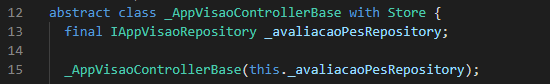
\includegraphics[scale=0.9]{Imagens/desenvolvimento/app_visao_controller.png}
    \end{center}
    \legend{Fonte: Autor.}
\end{figure}

Já os \emph{singletons} dos controladores, por sua vez, são recuperados nas telas,
como nota-se na linha 24 da \autoref{fig_pag_app_vis}.

\begin{figure}[htb]
    \caption{\label{fig_pag_app_vis}Recuperar \emph{Controller} na \emph{Page}.}
    \begin{center}
        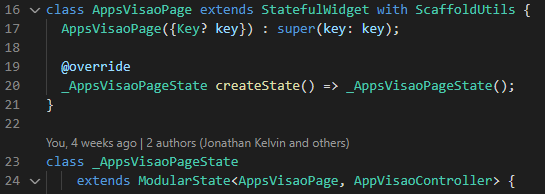
\includegraphics[scale=0.9]{Imagens/desenvolvimento/app_visao_page.png}
    \end{center}
    \legend{Fonte: Autor.}
\end{figure}